\chapter{Introduction}
\section{Market}
The global household robots market was valued at \$8.03 billion in 2021 and is expected to grow to \$32.9 billion by 2030 \cite{polarismarketresearchlastHouseholdRobotsMarket2022}. Major players in the market like Amazon Echo and Google Home all allow people to speak to the device just like they would to another person and command it to do simple tasks around the house. The major draw to these robots is automating repetitive tasks like scheduling reminders or household chores. Robots do not get bored of these tasks and also do not require wages, which reduces the overhead expense \cite{polarismarketresearchlastHouseholdRobotsMarket2022}. This is an example of human-robot interaction, which describes a class of research that studies how robots can better the lives of humans through means of collaboration or companionship \cite{cornellbowerscisHumanRobotInteraction2023}. However, natural human-robot interaction is a difficult challenge to tackle. It is unfortunately very difficult for robots to replicate human to human interactions. Recent developments in that area have been software focused, with OpenAI's ChatGPT generating realistic human speech. However, there is still potential in improving the physical aspect of the robots, namely their appearance. Many robots seem to lack a physical presence, opting for a more minimalist look. This is good for efficiency and reducing manufacturing costs, but it comes at the expense of reducing human-robot interaction. A person has nothing to focus on when they are talking to ``black box'' kinds of robotic assistants like Amazon Alexa or Google Home. Robot companies have sought to fix this issue with simulating a face with a screen. Robots like Aido and Zenbo, seen in Figure \ref{fig:aido-zenbo}, use an LCD to display various facial expressions. However, this lacks physicality and pales in comparison to a physical mechanism that is more tangible and natural to focus on. 

\begin{figure}[h]
    \centering
    \begin{subfigure}{0.4\linewidth}
        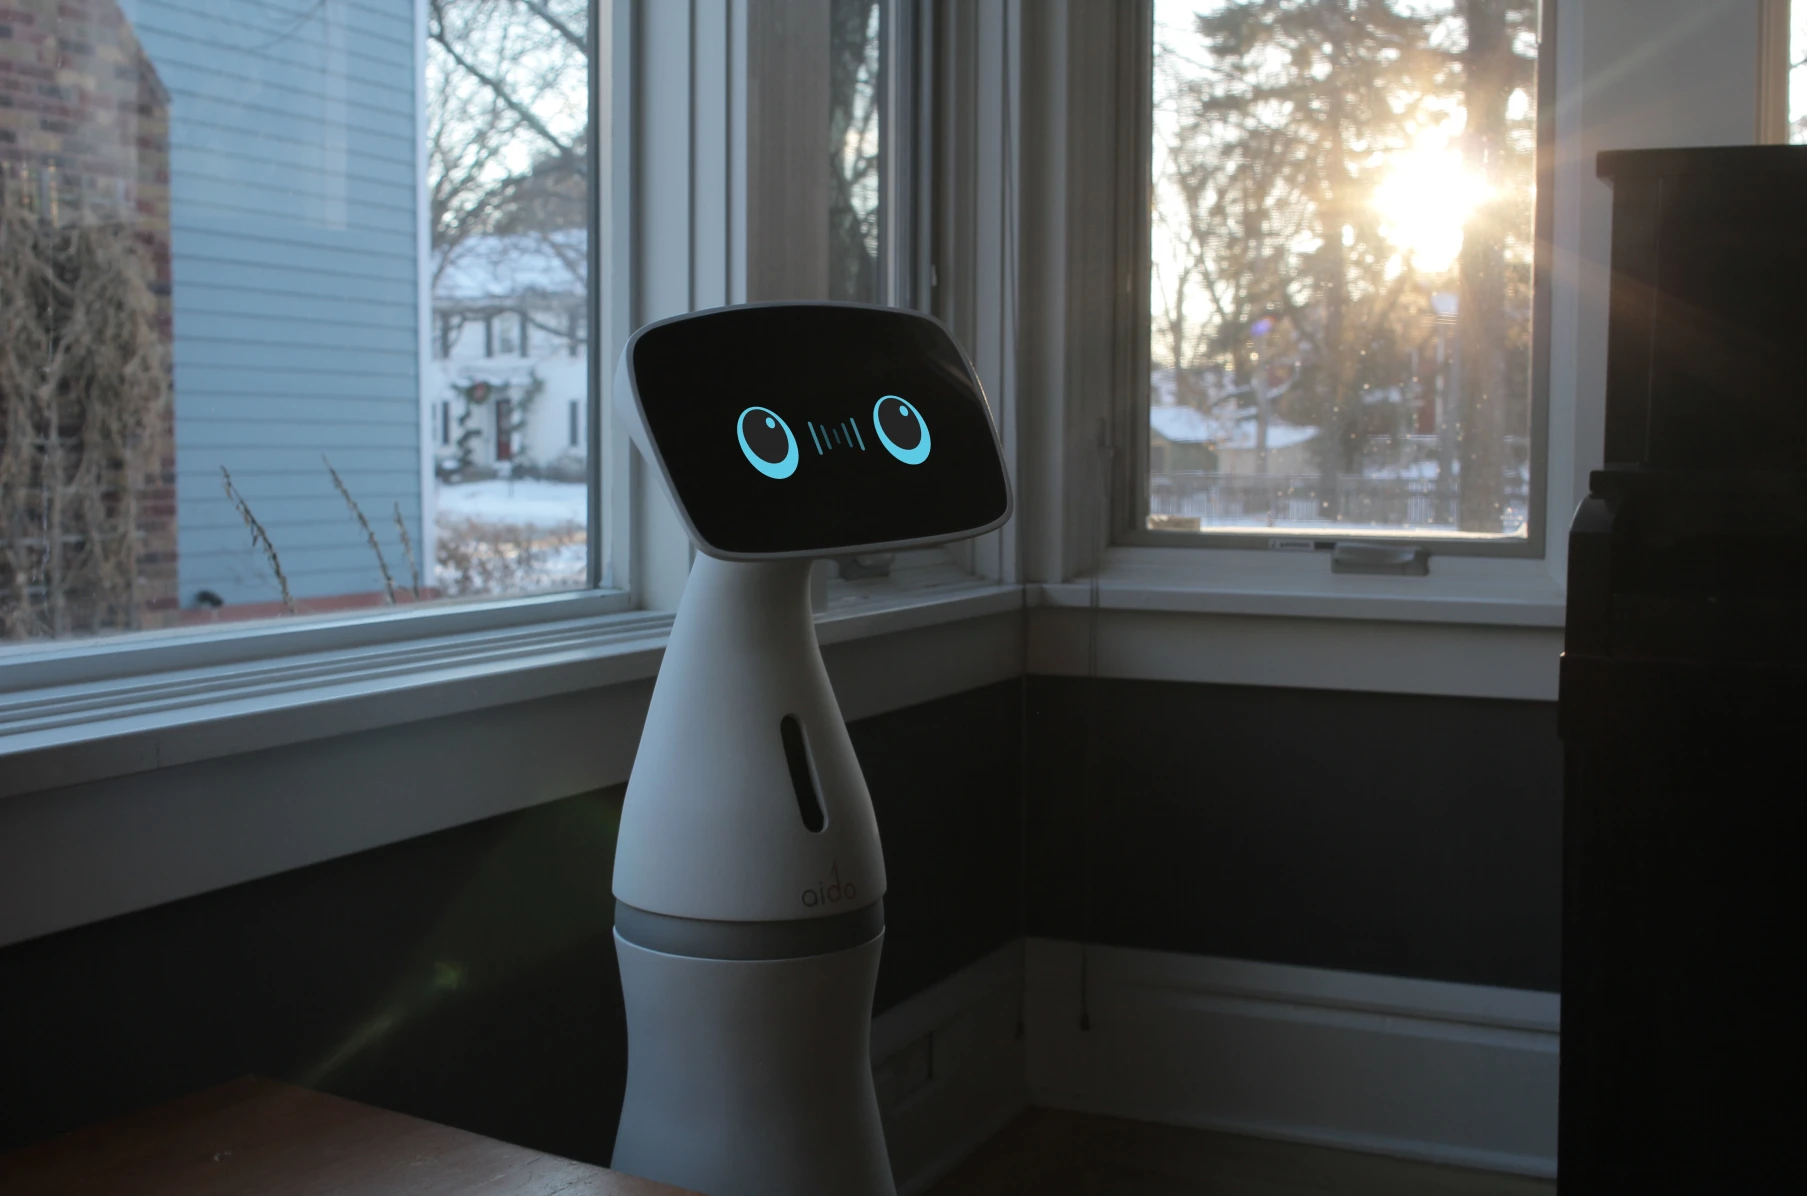
\includegraphics[width=\textwidth]{Thesis/ch1/aido.png}
        \caption{Aido robot. Courtesy of Ingen Dynamics Inc.}
    \end{subfigure}
    \begin{subfigure}{0.4\linewidth}
        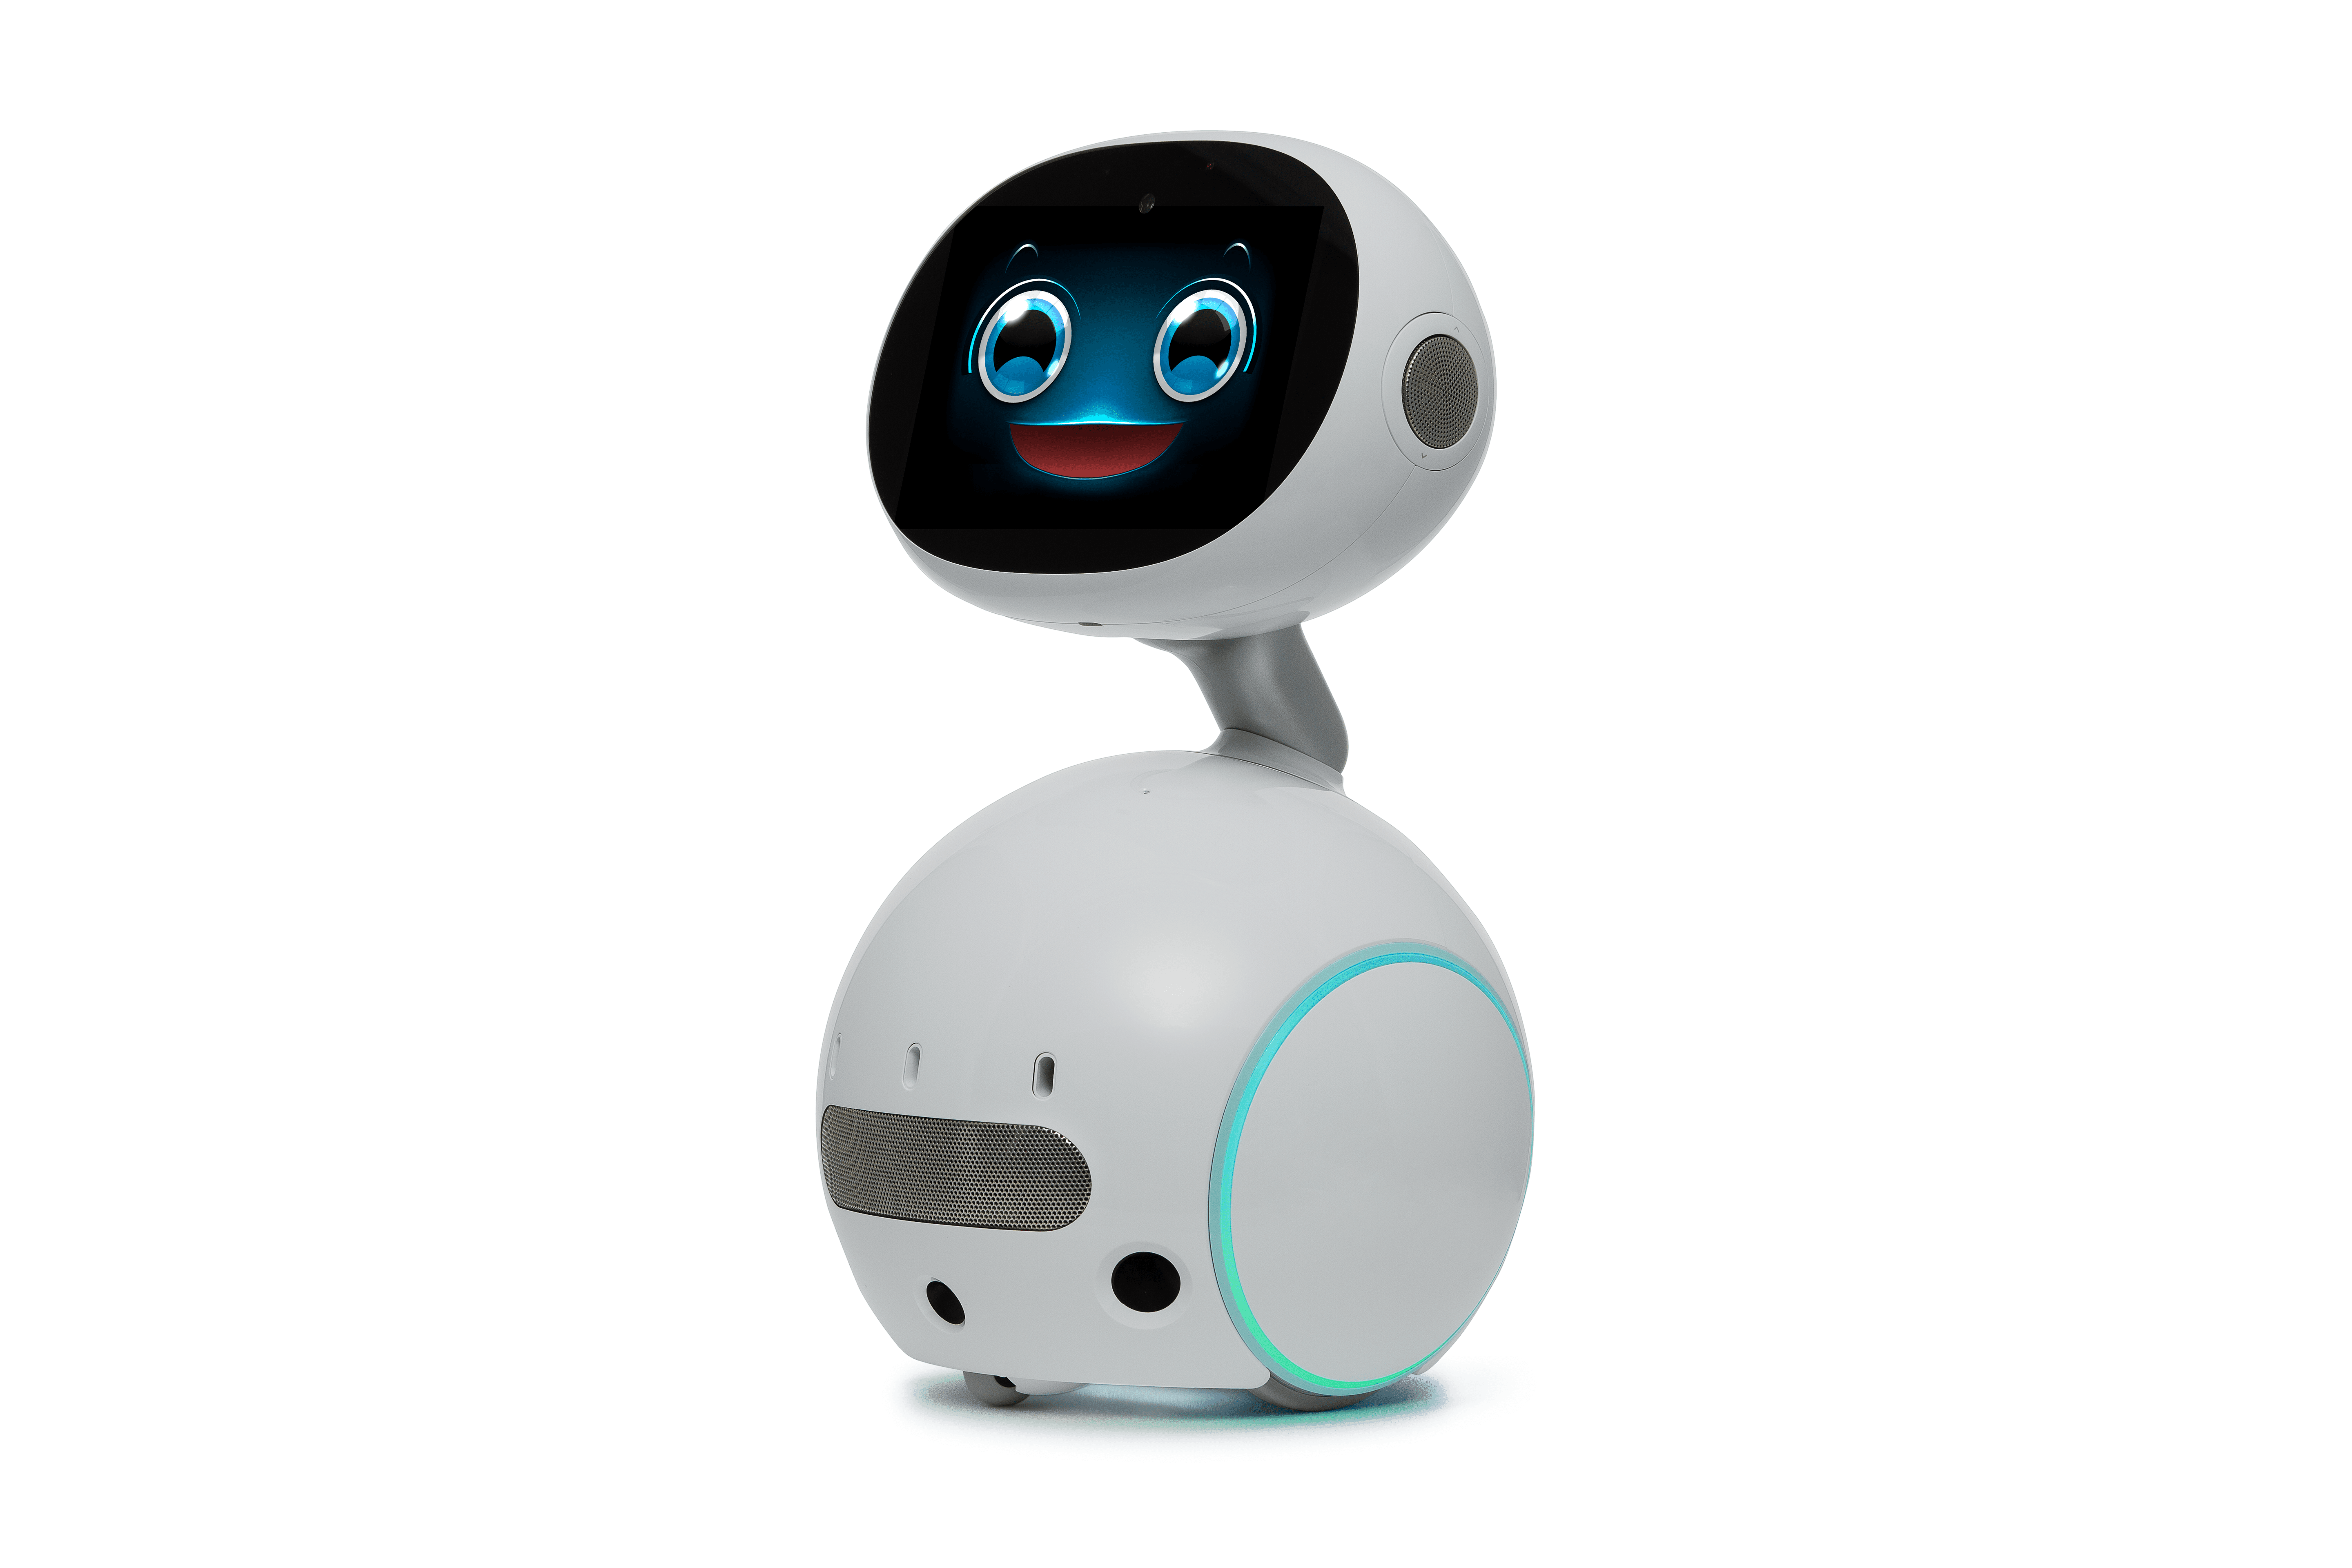
\includegraphics[width=\textwidth]{Thesis/ch1/zenbo-junior.png}
        \caption{Asus Zenbo robot. Courtesy of IEEE Spectrum.}
    \end{subfigure}
    \caption{Two examples of screen-based robot faces.}
    \label{fig:aido-zenbo}
\end{figure}

Eye contact is one of the most important parts of communication. It demonstrates that the other person in listening and valuing what is being said. If a human interacting with a robot cannot make eye contact with it while talking to it, it may lead them to believe it is not really listening. It also serves as a good indicator for when the robot is actively listening, providing the user with visual feedback. Therefore, this project's hypothesis is that adding a mechanical eye will allow the robot to be more friendly and approachable to humans.

\section{Design Goal}
The objective of this project is to design a mechanically actuated eye mechanism for use in human robot interaction. The goal is to have the eye make and maintain eye contact with the user by recognizing their face and tracking it as the user moves around it. Before getting into the specifics, it is important to note some areas that are considered out of scope for this project. The obvious choice would be to make a full face, with two eyes, nose, and mouth, with realistic movements and animations. However, given the limitations of time and budget, only the eye was specifically focused on in this project. Another limiting factor in this design is budget, using common consumer and hobby level electrical components. As such, the physical size of the project is constrained by the side of these cheap components. This is another reason why only the eye mechanism was the focus, as adding other supplementary mechanisms would certainly enhance the user experience, but without using custom components it is difficult to fit other mechanisms in such a compact space as a robot head.

\section{Existing Products}
There are a multitude of mechanical eye and face tracking camera projects on the internet. Numerous patents have been filed for mechanical representations of the human eye, such as one filed by Disney for use in their animatronic characters \cite{smootAnimatronicEyeElectromagnetic2019}. This patent uses fluid suspension and electromagnets to move the eye in a smooth manner. This approach is ultimately out of scope for this project, but still demonstrates that eye mechanisms are possible and have been done before. As for face tracking mechanisms, one product that came up in the preliminary research is the DJI Osmo 6 \cite{djiOsmoMobileUnfold2022}. It is a essentially a high-tech selfie stick, with a 3-axis stabilizing system that allows the user to insert their phone and focus on the subject. This is a sophisticated product, but the mechanism behind it is quite simple: there is a rotating motor for the 3 axes, and some sensors to detect the movement of the user and actuate the motors according to some control law that stabilizes the camera. This served as a basic outline of how this thesis would be completed, albeit with numerous simplifications. However, one thing that this design lacks is any physical presence. It is essentially a series of rods, opting for a minimal design. This may be good for economics, but for human-robot interaction this is not enough. More human elements would have to be allow people to empathize with the robot. Therefore, instead of just the stabilizing mechanism, research shifted focus to humanoid robots.

\section{Humanoid Robots}
One example of a humanoid robot is named Sophia from Hong Kong based company Hanson Robotics \cite{hansonroboticslastSophia2023}. This robot has a realistic human face, complete with synthetic skin and actuated facial expressions. A similar robot named Ameca by British Company Engineering Arts also has a very realistic face \cite{engineeredartslastAmeca2023}. This is very impressive, but something is still off about them. They almost approach a human appearance, but they fall short just slightly. On top of this, there are diminishing returns as a robot approaches human appearance, as it takes much more effort to perfect it. These ``creepy'' humanoid robots fall into what is known as the Uncanny Valley.
\begin{figure}[h]
    \centering
    \begin{subfigure}{0.3\linewidth}
        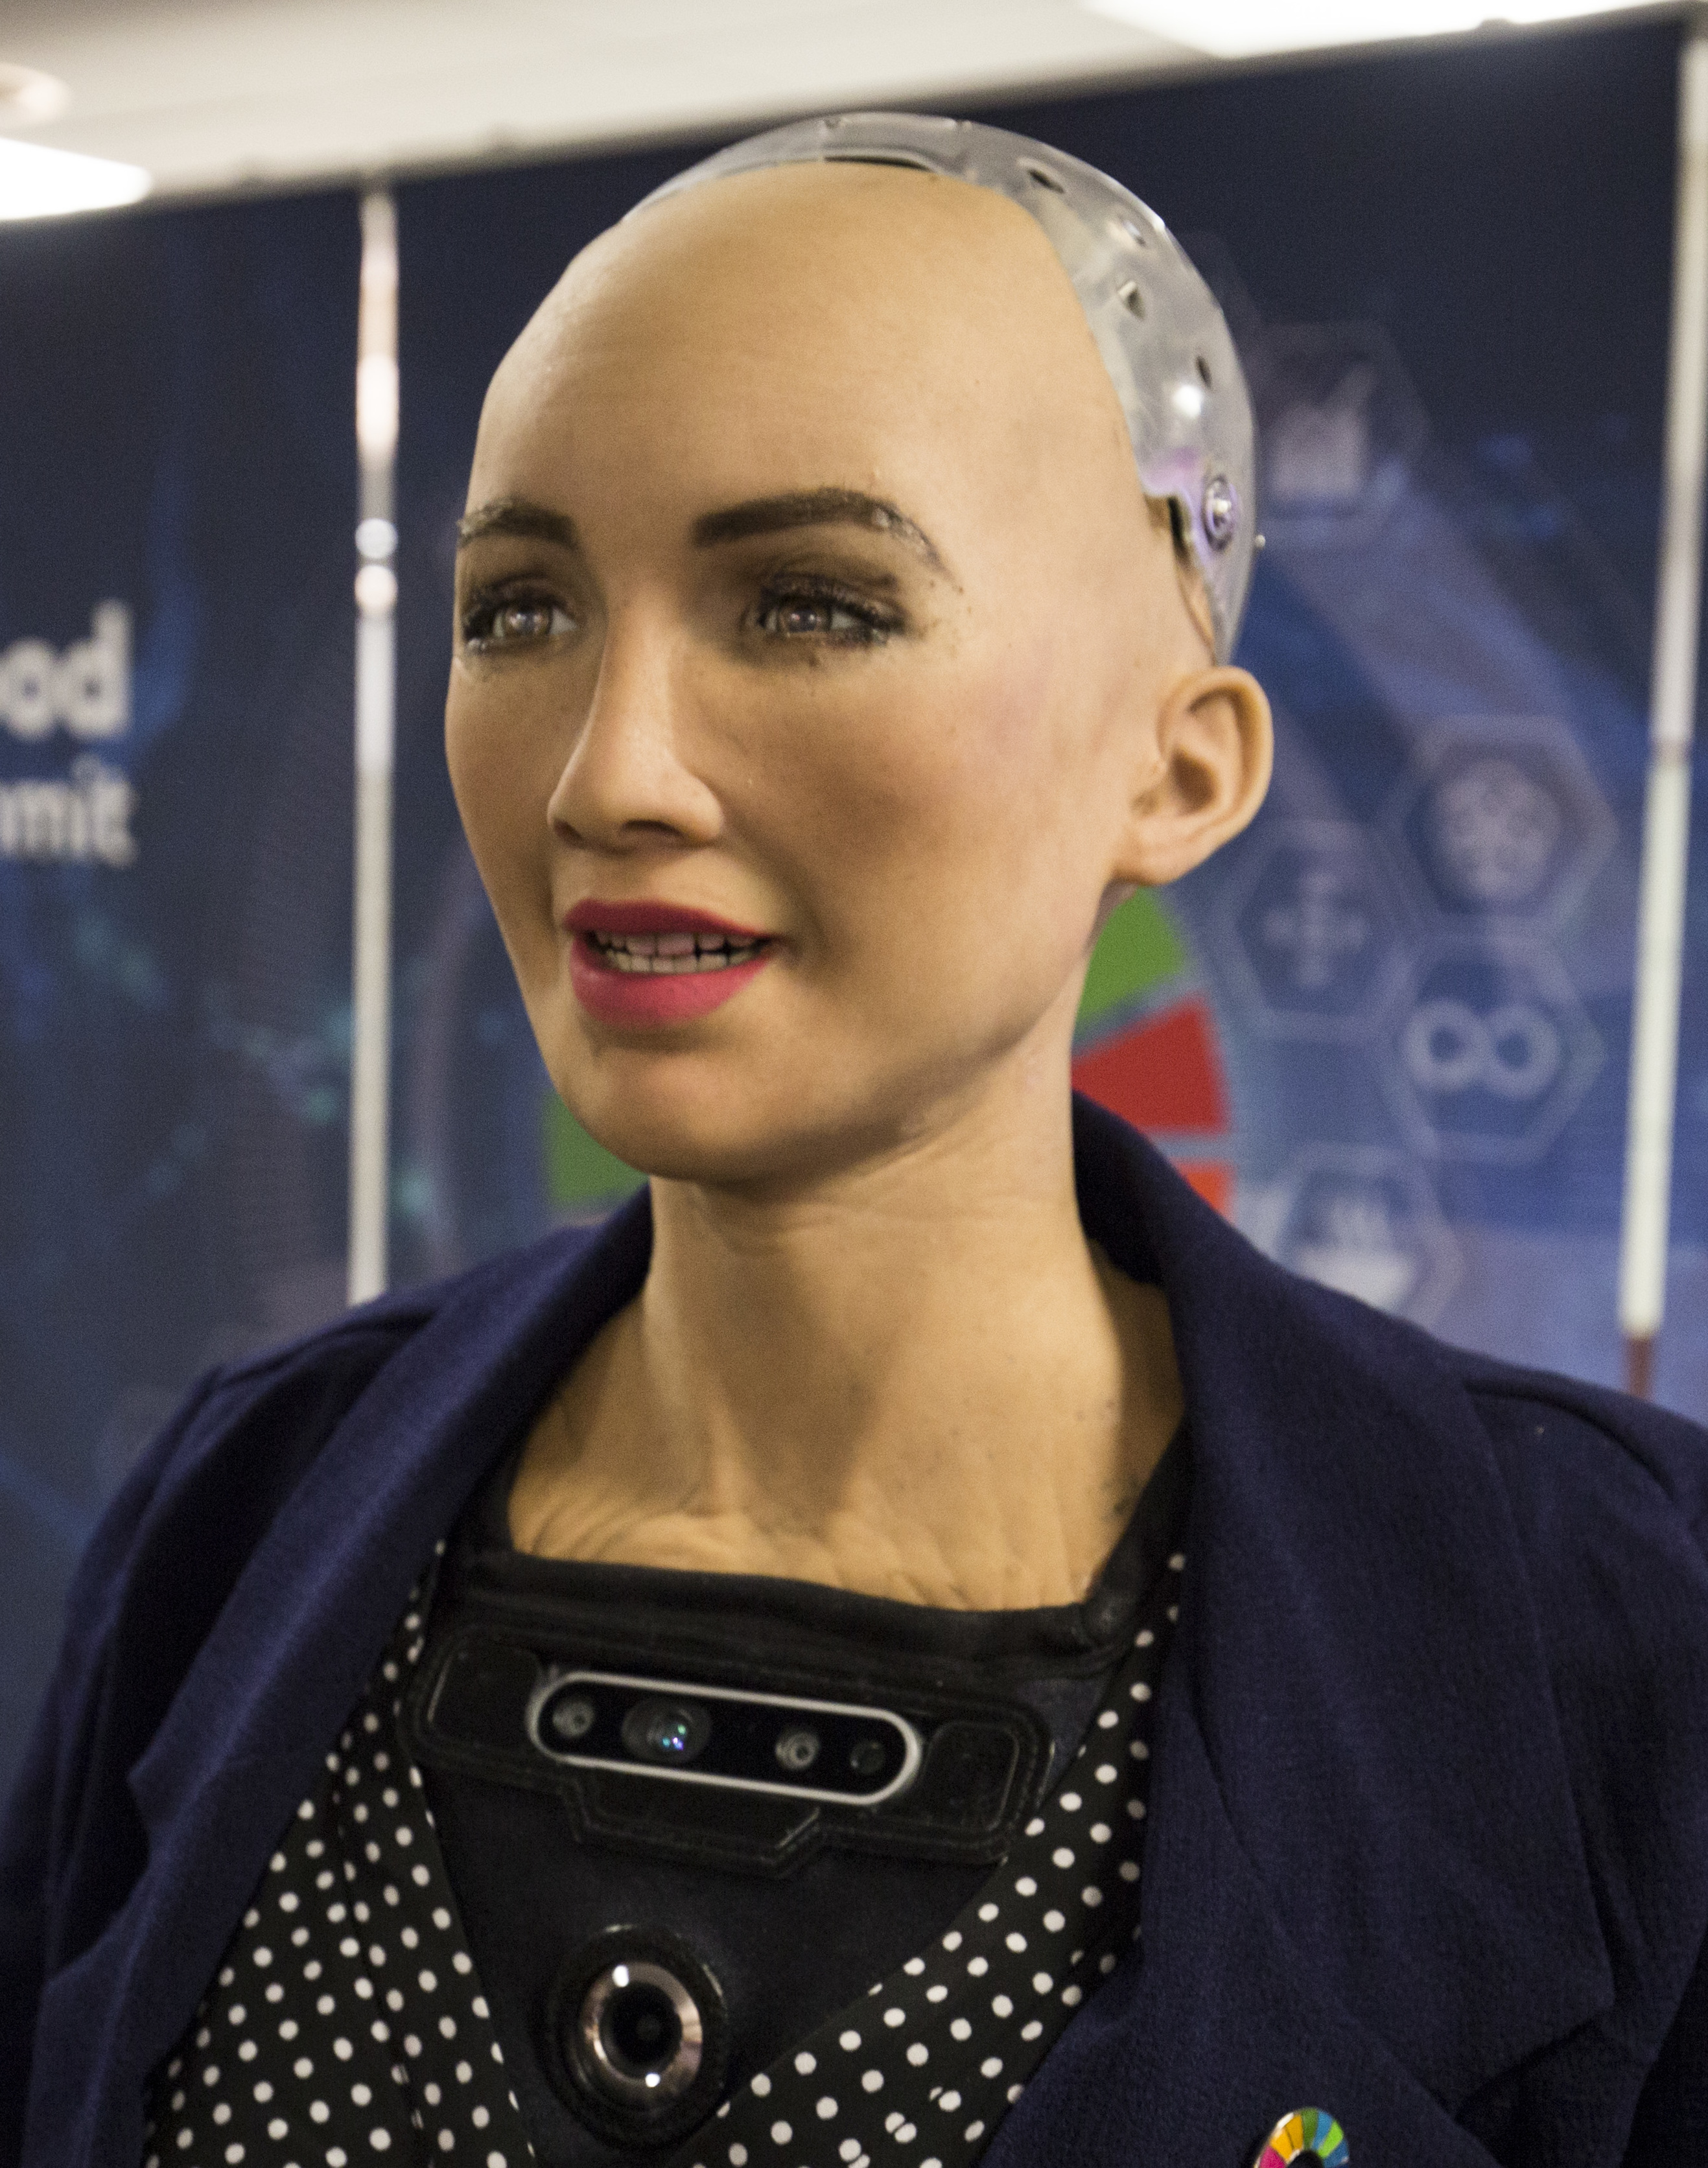
\includegraphics[width=\linewidth]{Thesis/ch1/sophia.jpg}
    \end{subfigure}
    \begin{subfigure}{0.3\linewidth}
        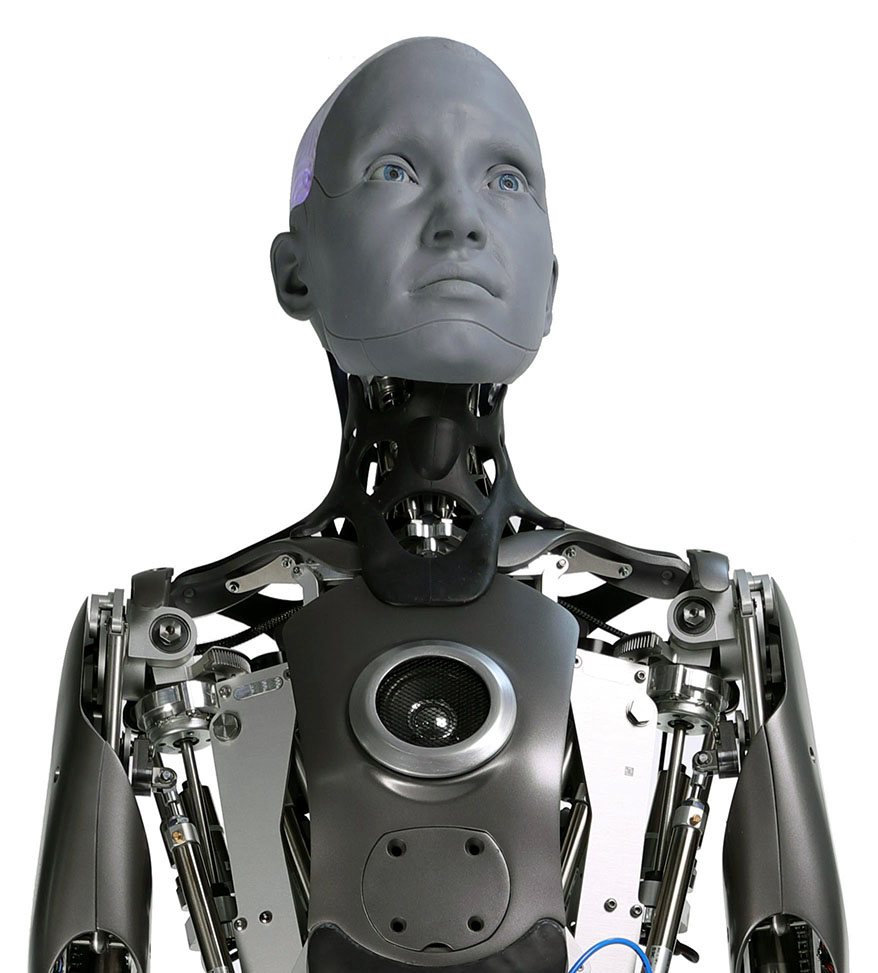
\includegraphics[width=\linewidth]{Thesis/ch1/Ameca_Generation_1.jpg}
    \end{subfigure}
    \caption{Two examples of humanoid robots on the market today.}
    \label{fig:humanoid}
\end{figure}

\subsection{The Uncanny Valley}
One of the guiding design principles of this project was based on the concept of the Uncanny Valley, first proposed by Masahiro Mori in his 1970 essay of the same title \cite{masahiromoriUncannyValleyOriginal2012}. The classic Uncanny Valley graph is shown in Figure \ref{fig:uncanny valley}, which illustrates how making a robot look more like a human can the affect a persons' affinity to it. Industrial robots are designed with functionality in mind, simply having a robotic arm or wheels. As more human-like qualities are added to a robot, like a cartoonish face or legs, peoples' affinity to it goes up. However, there comes a point when adding more human-like qualities where approaching a real human tilts the scale in the opposite direction. If a robot resembles a human very closely but is not perfectly, it falls into what is known as the Uncanny Valley. The person's affinity to the robot violently switches from empathy to aversion. This problem causes many humanoid robot designs, such as those shown in Figure \ref{fig:humanoid}, to appear creepy or unsettling to humans. This in turn has an effect on peoples' willingness to interact with them. Modern advances in humanoid robots seek to mitigate this issue by going further and further right on the Uncanny Valley graph. If a robot can have perfectly realistic facial expressions, movements, and materials, perhaps they can one day be indistinguishable from a human and escape the Uncanny Valley. In the present day however, technology is not there yet, so a more practical option is instead to target the left portion of the graph. If a robot could hit the peak before hitting the Uncanny Valley, it can maximize its appeal to humans without seeming creepy. Therefore, this project will be following this doctrine, where the robot will have human-like qualities, like a mechanical eye, but will not attempt to replicate human movement directly.


\begin{figure}[h]
    \centering
    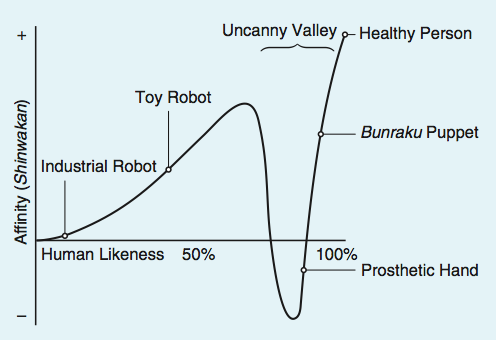
\includegraphics[width=0.6\linewidth]{Thesis/ch1/uncanny-valley.png}
    \caption{Uncanny Valley graph, courtesy of Masahiro Mori.}
    \label{fig:uncanny valley}
\end{figure}

\section{One-Eyed Characters}
While looking for design inspiration on how to make the robot more friendly, one commonality was identified across numerous examples. Many one-eyed character designs were seen as cute and friendly, with various examples being shown in Figure \ref{fig:one-eye}. A large inspiration for the aesthetic design of this project was a robot from the video game Portal 2, which were digitally animated but were very expressive for the low amount of joints and components in the design. In particular a YouTube video by the creator DJ Harrigan was an inspiration, where he recreated a character from this video game in real life, complete with actuated mechanisms and aesthetic appearances \cite{harriganPortalWheatleyReal2022}. This was important in establishing the feasibility of this project, as this project would have to accomplish something similar in a shorter time frame. Another inspiration for the design of the robot was the Pixar Lamp, named ``Luxo Jr.'', an animated desk lamp that appears in the logo at the beginning of Pixar films. The simplicity of the design is appealing, that with just a head, body and base, the lamp is able to have a physical presence and move around. Another YouTube creator created this recreation of the Pixar lamp, which uses an entire robotic arm and inverse kinematics to follow a face \cite{terranovaThisAdorableRobotic2015}. This is impressive for sure, but out of scope for this project. Still, it gave a good foundation for what the end product should look like and how it should interact with the user.

Research also seemed to indicate that scarier robots had two eyes, such as the Terminator robot pictured in Figure \ref{fig:terminator}. Perhaps they look too human, while one eyed robots appear more approachable because they show just enough human qualities without getting too close to the Uncanny Valley. This project proposes this as a novel approach to facilitating human-robot interaction. The mechanical eye mechanism will be one eyed rather than two eyed, and it is theorized that this would have a better effect on making a robot more approachable and accomplishing the design goal.
\begin{figure}[h]
\centering
\begin{subfigure}{0.2\textwidth}
    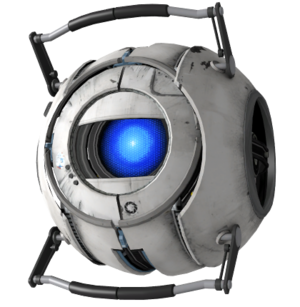
\includegraphics[width=\textwidth]{Thesis/ch1/300px-Wheatley.png}
    \label{fig:first}
\end{subfigure}
\hfill
\begin{subfigure}{0.2\textwidth}
    
\includegraphics[width=\textwidth]{Thesis/ch1/Mike_Wazowski.png}
    \label{fig:second}
\end{subfigure}
\hfill
\begin{subfigure}{0.4\textwidth}
    
\includegraphics[width=\textwidth]{Thesis/ch1/pixar_lamp.jpg}
    \label{fig:third}
\end{subfigure}
\caption{Various examples of approachable one-eyed characters.}
\label{fig:one-eye}
\end{figure}
\begin{figure}[h]
    \centering
    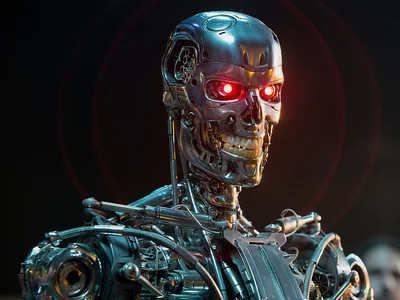
\includegraphics[width=0.5\linewidth]{Thesis/ch1/terminator.jpg}
    \caption{An example of a scary robot, courtesy of Paramount Pictures.}
    \label{fig:terminator}
\end{figure}